\section{Phase Transitions and Quantum Corrections}
\label{sec:quantum}

\begin{figure}
	\centering
	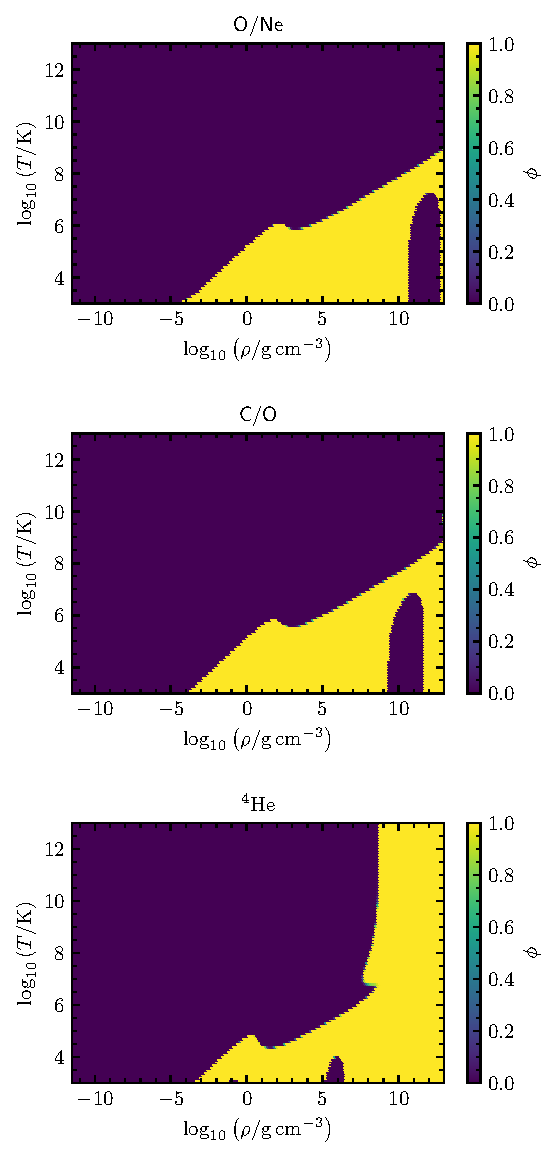
\includegraphics[width=0.45\textwidth]{3_phase.pdf}
	\caption{The phase $\phi$ is shown as a function of temperature and density for (upper) an equal-mass mixture of $^{16}\rm O$ and $^{20}\rm Ne$, (middle) an equal-mass mixture of $^{12}\rm C$ and $^{16}\rm O$, and (lower) pure $^{4}\rm He$.}
	\label{fig:3_phase}
\end{figure}

Figure~\ref{fig:3_phase} shows the \skye\ phase $\phi$ as a function of $\rho$ and $T$ for three different compositions.  At high temperatures and low densities the system is a liquid, and it crystallizes in the opposite limit.  This standard OCP-like phase transition that occurs at approximately constant $\langle \Gamma \rangle$ is discussed in the main text.  However, Figure~\ref{fig:3_phase} displays additional structure in the phase, which we determined to be primarily related to the quantum correction terms in the free energy.  These features likely reflect limitations in the assumed prescriptions.

At high densities for the lightest elements ($\mathrm{H}$ and $\mathrm{He}$), quantum corrections dominate and favor the solid phase up to high temperatures.  While a self-consistent consequence of the adopted inputs, we suspect this feature is spurious.  However, as $^{4}\mathrm{He}$ and $^{1}\mathrm{H}$ are likely to have fused into heavier elements long before reaching these densities in typical astrophysical applications, 
we have done nothing to suppress this solidification in \skye.

At high densities and at low temperatures, quantum corrections dominate and cause the system to melt.
This occurs at lower densities and temperatures for lower-mass lower-charge species: $10^{10}\,\mathrm{g\,cm^{-3}}$ for O/Ne, $10^{8}\,\mathrm{g\,cm^{-3}}$ for C/O, and $10^4\,\mathrm{g\,cm^{-3}}$ for $^{4}\mathrm{He}$).
%
A similar effect has been seen in Monte Carlo calculations and analytic calculations~\citep{1993ApJ...414..695C,PhysRevB.18.3126,PhysRevLett.76.4572}.
In those studies the Lindemann criterion was used to compute the quantum melt line, but the result has a rather different topology from the phase  boundary we see (Figure~\ref{fig:C_phase}).
In particular we see the quantum melt only for a finite density range, whereas they predict it for all densities above a cutoff.
The latter is more in line with our understanding of the physics of quantum melting, namely that it is driven by the zero-point energy of ions and so should only increase with increasing density.
We therefore suspect that the topology of this melt region reflects limitations in our prescriptions for the OCP quantum corrections.

Moreover the temperature and density scale involved is rather different from Lindemann criterion calculations~\citep{1993ApJ...414..695C,PhysRevB.18.3126,PhysRevLett.76.4572}, though interestingly the \emph{scaling} of these scales matches those from the Lindemann criterion.
The melt line is predicted to peak around $k_{\rm B} T \approx 6\times 10^{-5}\,\mathrm{Ry}_{j}$, where
\begin{align}
	\mathrm{Ry}_{j} = (Z_{j} e)^4 m_{j} / 2 \hbar^2
\end{align}
is the ionic Rydberg.
Instead we see a peak near $6\times 10^{-6}\,\mathrm{Ry}_{\rm ion}$.
Likewise the melt line is predicted to peak in temperature when the dimensionless ion sphere radius
\begin{align}
	r_{s,j} \equiv \left(\frac{3 m_j}{4\pi \rho}\right)^{1/3}  \frac{m_j (Z_j e)^2}{\hbar^2}
\end{align}
is of order $200$, and we see the peak around $1200$.

\begin{figure}
	\centering
	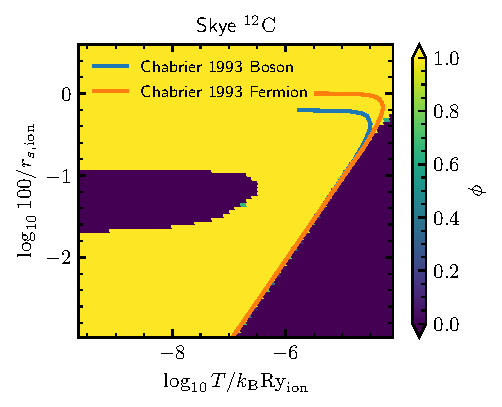
\includegraphics[width=0.45\textwidth]{C_phase.pdf}
	\caption{The phase $\phi$ is shown as a function of temperature in units of $\mathrm{Ry}_{\rm ion}$ and reciprocal ion spacing measured by $100/R_{S,\rm ion}$. The melt lines of~\citet{1993ApJ...414..695C} for bosons (blue) and fermions (orange) are over-plotted for comparison. This calculation was done for pure $^{12}\mathrm{C}$, but the choice of units means the results are universal for any pure ionic system.}
	\label{fig:C_phase}
\end{figure}


Overall the disagreement between \skye\ and calculations based on the Lindemann criterion suggests caution in interpreting these results.
This disagreement may be caused by our use of the fit by~\citet{2019MNRAS.490.5839B} beyond its range of validity, which is confined within the dark blue triangle at the lower right corner of Figure~\ref{fig:C_phase}.
These results are, however, a completely self-consistent consequence of the input physics
so we have not done anything to impede quantum melting in \skye.

